\section{Introduction}
\subsection{Le Cerfacs}\label{sec:intro}

Le Cerfacs (Centre Européen de Recherche et de Formation Avancée en Calcul Scientifique) est un centre de recherche spécialisé dans le calcul scientifique et la simulation numérique. Créé en 1987, il travaille pour ses actionnaires (Airbus Group, Cnes, EDF, Météo France, Onera Safran et Total) à la résolution de problèmes scientifiques et techniques liés au climat, à l'aéronautique, au spatial et à l'environnement par la simulation numérique nécessitant une puissance de calcul élevée. Il travaille également en partenariat avec le CNRS, l'Irit, le CEA ainsi que l'Inria.


Le personnel du Cerfacs est réparti en équipes:
\begin{itemize}
\item Algorithmes parallèles
\item Aviation \& environnement
\item Informatique et Support Utilisateur (CSG)
\item Modélisation du climat
\item Mécanique des fluides (CFD)
\end{itemize}

\subsubsection{L'équipe CFD}
L'équipe CFD (\textit{Computational Fluid Dynamics: mécanique des fluides numérique}) est la plus grosse équipe du Cerfacs et c'est en son sein que j'ai réalisé mon stage. Elle se concentre sur le développement de méthodes numériques permettant la simulation des écoulements et les applique aux avions, fusées, moteurs, turbines, etc. Ces méthodes permettent ensuite d'étudier les mouvements de fluides et leurs effets par la résolution d'équations régissant de tels fluides. L'avantage des simulations mises en place est grand pour l'industrie; elles permettent d'étudier des phénomènes complexes pour un coût très inférieur à des expériences "réelles".

Bénédicte CUENOT, une des chef de projet de l'équipe, m'encadrait pour la partie physique de mon stage.


\subsubsection{L'équipe CSG}
L'équipe CSG (\textit{Computer Support Group}) s'occupe de la gestion des infrastructures informatiques et des moyens matériels mis à la disposition des différentes équipes. Elle fournit également son expertise aux chercheurs pour qu'ils puissent exploiter au mieux les outils et le matériel disponibles.
Dans le cadre de mon stage, j'ai surtout eu contact avec Mme Isabelle D'AST, ingénieur Logiciel HPC. C'est elle qui m'a conseillé sur toute la partie HPC (\textit{High Performance Computing}) et plus généralement, sur tous les problèmes liés à la programmation.

\subsection{Le stage}
\subsubsection{NTMIX\_CHEMKIN}
Mon stage portait sur NTMIX\_CHEMKIN, un des codes de simulation développé par l'équipe CFD. C'est un solveur d'écoulements réactifs (``écoulements dans lesquels il y a des réactions chimiques'') en 2D s'appuyant sur une approche DNS (Direct Numerical Simulation). Il est couplé avec la librairie CHEMKIN qui permet la simulation de la chimie complexe. Ce code est utilisé pour étudier la structure chimique des flammes et leur comportement en présence d'un écoulement dynamique (combustion turbulente).\cite{cerfacs}



Une simulation numérique directe (DNS: Direct Numerical Simulation) est une simulation dans laquelle les équations de Navier-Stokes (équations décrivant le mouvement des fluides visqueux) sont résolues numériquement sans aucun modèle de turbulence. Cependant, le coût d'une telle simulation est très élevé. Il est actuellement impossible de résoudre des problèmes industriels avec ce type de simulation. Elle présente cependant un intérêt en recherche fondamentale. Grâce à la DNS, il est possible de faire des ``expériences numériques'' et d'en extraire des informations difficilement récupérables en laboratoire.\cite{cfd-online-DNS}


\subsubsection{Objectifs}
Comme vu précedemment, le coût d'une simulation réalisée par NTMIX\_CHEMKIN est très élevé. Son utilisation était donc restreinte au cas en bidimensionnel, mais l'évolution des machines de calcul parallèle permet aujourd'hui d'utiliser une version tridimensionnelle à des coûts raisonnable.


Le développement d'une version 3D est motivé par le fait que NTMIX\_CHEMKIN utilise une librairie permettant de prendre en compte les cinétiques complexes des éléments chimiques (CHEMKIN), contrairement à NTMIX\_3D, un autre logciel de simulation développé au Cerfacs, déjà en 3D mais n'utilisant pas de chimie complexe. Le portage en 3D permettra donc d'observer des phénomènes complexes ne pouvant pas forcément être obtenus avec d'autres méthodes de simulation.


Cependant, une simulation DNS n'utilise pas de modèle de turbulence. Il sera nécessaire de paralléliser la version 3D de NTMIX\_CHEMKIN pour permettre au code de tourner sur de grands maillages ($\approx 10^9$ points) en un temps raisonnable.


\paragraph{}Pour atteindre ces objectifs, il sera nécessaire de procéder par étapes; dans un premier temps, je devrais moderniser le code avant de développer une version 3D de celui-ci. Cette partie permettra d'obtenir une première version tridimensionnelle, testée et validée de NTMIX utilisant des concepts de programmation plus récents et sera présentée en section \ref{sec:part1}

Dans la section \ref{sec:part2}, je m'intéresserai au développement d'une version parallèle de l'application et aux modifications induites par une telle version. Cette version devra permettre d'exécuter des simulations sur des machines parallèles.

Enfin, dans une dernière partie (section \ref{sec:part3}), je mesurerai les performances de NTMIX sur les calculateurs internes du Cerfacs afin d'essayer de tirer les meilleurs performances possibles.

\paragraph{}A terme, la version finale de NTMIX permettra de faciliter la compréhension de phénomènes complexes liés à la mécanique des fluides et pourra aboutir à la rédaction de publications scientifiques par les chercheurs présents au Cerfacs.

\subsection{Présentation de la mécanique des fluides}
\subsubsection{Mécanique des fluides numérique}
La \textbf{mécanique des fluides} est l'étude du comportement des fluides (liquides, gaz et plasma) lorsqu'ils sont en mouvement et est un domaine actif de recherche notamment en mécanique des fluides numérique (\textit{ou CFD}). Ce sous-domaine s'intéresse à l'étude des mouvements par la \textbf{résolution numérique} des équations régissant les fluides. Les équations les plus utilisées sont:

\begin{itemize}
\item les équations d'Euler dans le cas des fluides parfaits; elle ne prennent pas en compte la viscosité et la conductivité thermique
\item les équations de Navier-Stokes dans le cas des fluides newtoniens
\end{itemize}


Dans le cas de NTMIX, ce sont les équations de Navier-Stokes; équations aux dérivées partielles qui sont résolues.

Cependant, la mécanique des fluides numérique se base sur des versions discrétisées de ces équations. Pour NTMIX, le domaine de calcul (espace) est divisé en volumes élémentaires (discrétisation spatiale) selon une approche structurée (maillage structuré) qui consiste à découper l'espace en cellules régulièrement espacées selon toutes les directions du domaine.


\subsubsection{Modèle de turbulence}
Dans un écoulement turbulent, des tourbillons instables apparaissent à toutes les échelles et interagissent entre eux. Pour pouvoir simuler un tel comportement, il existe 3 approches différentes:

\begin{itemize}
\item la méthode de simulation directe (\textit{DNS: Direct Numerical Simulation}): elle consiste à utiliser un maillage plus fin que le plus petit tourbillon attendu (fig. \ref{fig:dns})
\item la simulation des grandes échelles (\textit{LES: Large Eddy Simulation}): un modèle de turbulence est utilisé pour les plus petits tourbillons, permettant ainsi d'utiliser un maillage plus grossier (fig. \ref{fig:les})
\item le moyennage temporel des équations de Navier-Stokes (\textit{RANS: Reynold Averaged Navier-Stokes Simulation})
\end{itemize} 


\begin{figure}[ht]
  \centering
  \begin{subfigure}[b]{0.5\textwidth}
    \centering
    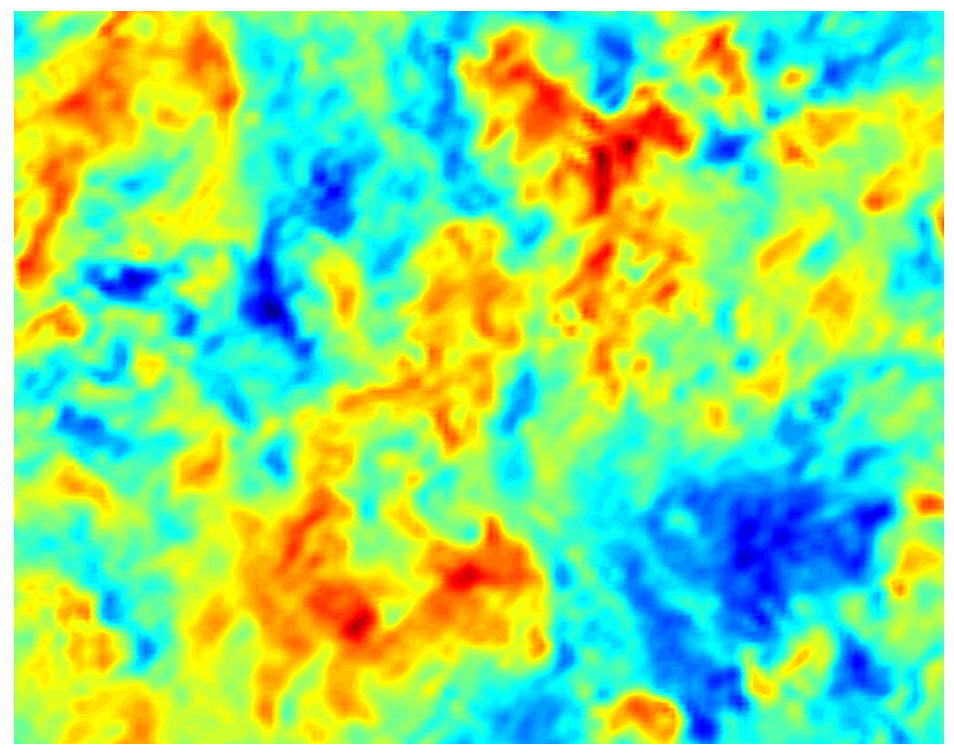
\includegraphics[scale=0.35]{figures/DNS_Velocity_Field.png}
    \caption{\label{fig:dns} Simulation des turbulences (DNS)}
  \end{subfigure}%
  ~
  \begin{subfigure}[b]{0.5\textwidth}
    \centering
    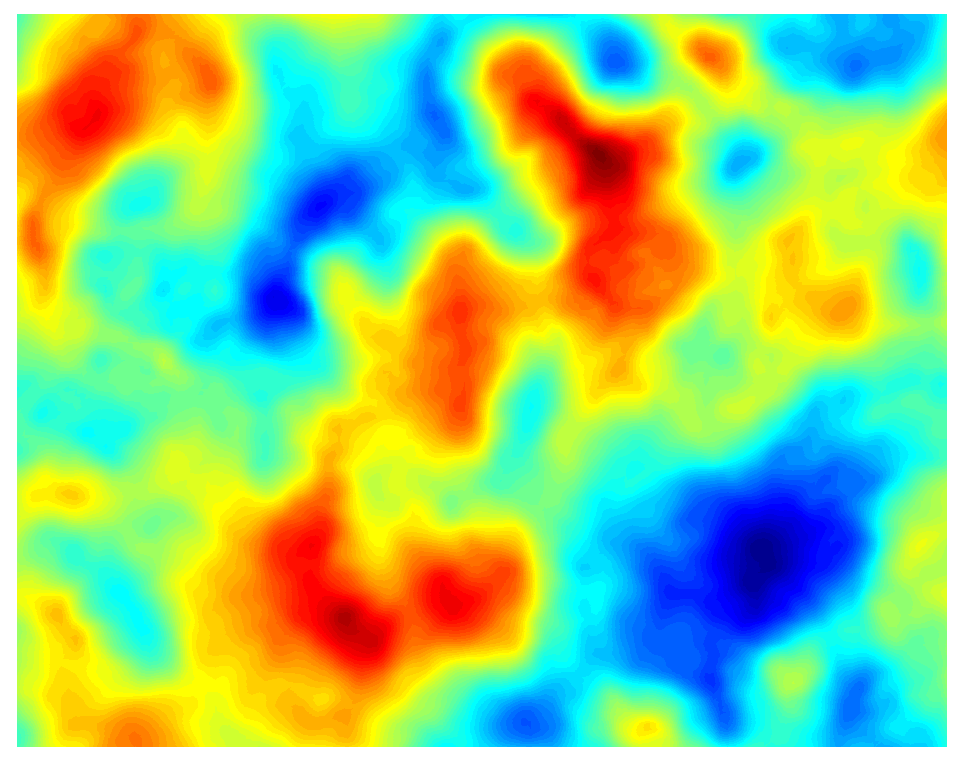
\includegraphics[scale=0.35]{figures/DNS_Filtered_Velocity_Field_Large.png}
    \caption{\label{fig:les} Simulation des grandes turbulences (LES)}
  \end{subfigure}
\end{figure}

L'approche DNS est donc la plus coûteuse en terme de puissance de calcul nécessaire étant donné qu'aucun modèle de turbulence n'est utilisé contrairement à la méthode LES qui ne simule que les tourbillons les plus grands, les petits tourbillons étant seulement modélisés. Les domaines d'applications de ces différentes méthodes sont donc différents; l'approche DNS est plutôt réservée à la recherche du fait des coûts élevés de telles simulations tandis que les méthodes LES et RANS sont plus adaptées à un contexte industriel.


\subsubsection{Vocabulaire lié à la CFD}

\begin{itemize}
\item Variables conservatives: ce sont les variables utilisées dans la simulation et qui sont soumises aux lois de conservation; conservation de l'énergie (masse) et conservation de la quantité de mouvement. Les variables conservatives se rapporteront donc ici à la densité, l'énergie et les vitesses selon toutes les directions.
\item Champ: c'est l'association d'une valeur d'un paramètre à un point de l'espace ou du maillage. Il existe des \textbf{champs scalaires} qui associent une valeur (densité, pression, etc.) à chaque point et des \textbf{champs vectoriels} qui associent un vecteur (vitesse) à chaque point de l'espace.
\item Gradient: c'est une opération réalisée sur un champ. C'est une généralisation de la dérivée pour une fonction à plusieurs variables.

\end{itemize}
